%% DCBA: Dual-Chain Blockchain Architecture for Secure,
%% Priority-Aware, UAV-Enabled Pharmaceutical Delivery
%% ACM SIGPLAN Proceedings Template

\documentclass[sigplan,screen,review=false]{acmart}

%% --- Package imports ---
\usepackage{booktabs}
\usepackage{multirow}
\usepackage{array}
\usepackage{xcolor}
\usepackage{listings}
\usepackage{algorithm}
\usepackage{algpseudocode}
\usepackage{graphicx}
\usepackage{tikz}
\usepackage{pgfplots}
\pgfplotsset{compat=1.18}
\usepackage{hyperref}
\usepackage{amsmath}
\usepackage{amssymb}
\usepackage{balance}

%% --- Listings style for Solidity ---
\definecolor{codegreen}{rgb}{0,0.5,0}
\definecolor{codegray}{rgb}{0.5,0.5,0.5}
\definecolor{codeblue}{rgb}{0,0,0.7}
\definecolor{backcolour}{rgb}{0.97,0.97,0.97}

\lstdefinelanguage{Solidity}{
  keywords={pragma,solidity,contract,function,returns,public,view,pure,
            mapping,address,uint256,uint8,bool,bytes32,string,memory,
            struct,event,emit,require,modifier,constructor,interface,
            enum,if,else,return,new,delete,import,using,for},
  keywordstyle=\color{codeblue}\bfseries,
  comment=[l]{//},
  morecomment=[s]{/*}{*/},
  commentstyle=\color{codegreen}\itshape,
  stringstyle=\color{red},
  morestring=[b]",
  sensitive=true
}
\lstset{
  language=Solidity,
  backgroundcolor=\color{backcolour},
  basicstyle=\ttfamily\footnotesize,
  breakatwhitespace=false,
  breaklines=true,
  captionpos=b,
  frame=single,
  rulecolor=\color{gray!30},
  numberstyle=\tiny\color{codegray},
  numbers=left,
  numbersep=5pt,
  showspaces=false,
  showstringspaces=false,
  tabsize=2
}

%% --- ACM metadata ---
\acmConference[CONF'26]{ACM Conference on Blockchain and Distributed Systems}{2026}{Dhaka, Bangladesh}
\acmYear{2026}
\copyrightyear{2026}

%% -------------------------------------------------------------------
\begin{document}

\title{DCBA: A Dual-Chain Blockchain Architecture for Secure,\\
       Priority-Aware, UAV-Enabled Pharmaceutical Delivery}

\author{Author One}
\affiliation{%
  \institution{Bangladesh University of Engineering and Technology}
  \department{Department of Computer Science and Engineering}
  \city{Dhaka}
  \country{Bangladesh}
}
\email{author1@buet.ac.bd}

\author{Author Two}
\affiliation{%
  \institution{Bangladesh University of Engineering and Technology}
  \department{Department of Computer Science and Engineering}
  \city{Dhaka}
  \country{Bangladesh}
}
\email{author2@buet.ac.bd}

\author{Author Three}
\affiliation{%
  \institution{Bangladesh University of Business and Technology}
  \department{Department of Computer Science and Engineering}
  \city{Dhaka}
  \country{Bangladesh}
}
\email{author3@bubt.edu.bd}

%% -------------------------------------------------------------------
\begin{abstract}
The global pharmaceutical supply chain faces a dual crisis: counterfeit
and substandard medicines cause an estimated one million deaths annually,
while last-mile delivery of time-critical medications remains
chronically inadequate in regions with constrained infrastructure.
Unmanned Aerial Vehicles (UAVs) offer a compelling solution to the
delivery problem but introduce new accountability and identity risks
when deployed without a secure operational framework.

This paper presents \textbf{DCBA} (Dual-Chain Blockchain Architecture),
a novel system that integrates two purpose-specific blockchain networks
--- a Patient Data Chain (PDC) built on Ethereum Proof-of-Authority and
a UAV Operational Chain (UOC) built on Hyperledger Fabric --- to
simultaneously address pharmaceutical supply chain integrity, patient
data sovereignty, and priority-aware drone delivery logistics. The two
chains communicate through \textbf{SC-7}, a cross-chain oracle bridge
providing replay-safe prescription verification.

DCBA introduces six original contributions: (1) a dual-chain
architecture that resolves the fundamental tension between patient
privacy and UAV operational throughput; (2) hardware-bound W3C
Decentralised Identifiers (DIDs) for UAVs that tie device identity to
physical MAC address, preventing impersonation; (3) a two-phase Drone
Capability Score (DCS) algorithm using Bloom filter pre-screening and
ECDSA verification, achieving selection in 8.37~ms for 100-drone fleets
--- 94\% below the 140~ms target; (4) sanitizable signature-based
medical records preserving Trusted Authority integrity during Healthcare
Provider amendments; (5) a Priority-Aware Routing System (PARS) with
four clinically grounded urgency tiers and on-chain SLA enforcement;
and (6) patient-sovereign encryption where records are mathematically
inaccessible to all parties except the patient.

The full system is implemented across seven Solidity smart contracts and
two Hyperledger Fabric Go chaincodes, validated by 86 automated tests
with zero failures, and benchmarked using Hyperledger Caliper. The
oracle bridge achieves a relay latency of 16~ms. All 10 adversarial
security test cases are blocked without false negatives.
\end{abstract}

%% -------------------------------------------------------------------
\begin{CCSXML}
<ccs2012>
 <concept>
  <concept_id>10002978.10002997.10002998</concept_id>
  <concept_desc>Security and privacy~Distributed systems security</concept_desc>
  <concept_significance>500</concept_significance>
 </concept>
 <concept>
  <concept_id>10010520.10010521.10010537.10010538</concept_id>
  <concept_desc>Computer systems organization~Peer-to-peer architectures</concept_desc>
  <concept_significance>300</concept_significance>
 </concept>
 <concept>
  <concept_id>10010147.10010919.10010172</concept_id>
  <concept_desc>Computing methodologies~Distributed computing methodologies</concept_desc>
  <concept_significance>300</concept_significance>
 </concept>
</ccs2012>
\end{CCSXML}
\ccsdesc[500]{Security and privacy~Distributed systems security}
\ccsdesc[300]{Computer systems organization~Peer-to-peer architectures}
\ccsdesc[300]{Computing methodologies~Distributed computing methodologies}

\keywords{blockchain, dual-chain architecture, UAV delivery, pharmaceutical supply chain,
          smart contracts, Hyperledger Fabric, Ethereum, cross-chain oracle,
          Drone Capability Score, Priority-Aware Routing}

\maketitle

%% ===================================================================
\section{Introduction}
\label{sec:intro}

\subsection{Background and Motivation}

Modern pharmaceutical supply chains span dozens of intermediaries ---
manufacturers, distributors, wholesalers, pharmacies, hospitals, and
patients --- across national and international borders. The opacity of
these multi-tier systems creates fertile ground for fraud,
counterfeiting, and diversion. The global trade in falsified medicines
is estimated to generate between USD~75 billion and USD~200 billion
annually~\cite{who2017falsified}. In Bangladesh, where the Directorate
General of Drug Administration (DGDA) oversees over 257 licensed
pharmaceutical manufacturers, manual and paper-based record systems
make real-time authentication of drug provenance practically
impossible~\cite{dgda2022annual}.

Beyond supply chain integrity, the delivery of medications to
patients --- particularly in urgent clinical contexts --- presents a
separate but equally critical failure mode. In Bangladesh, population
density in Dhaka exceeds 44,000~persons per km$^2$ and rural areas
face chronic healthcare access deficits. Conventional ground-based
delivery cannot meet the response time requirements of life-critical
medications: insulin for hypoglycaemia, epinephrine for anaphylaxis,
or anti-arrhythmics for a cardiac event must arrive within minutes.

UAVs have demonstrated deliveries in clinical settings across Rwanda,
Ghana, and the United States~\cite{zipline2022report,thiels2015uav}.
However, deploying UAVs in a pharmaceutical context without a secure,
auditable framework introduces serious risks: cloned UAV identities can
intercept deliveries; unverified prescriptions can enable drug
diversion; and the absence of an immutable GPS trail eliminates chain
of custody accountability.

Blockchain technology, with its properties of immutability,
decentralisation, and cryptographic auditability, presents the natural
technological foundation for addressing both problems simultaneously.
However, existing blockchain deployments in healthcare reveal a
fundamental architectural conflict: patient medical data demands strong
privacy and permissioned access --- properties best served by a private
blockchain. UAV operational data demands high throughput and
IoT-optimised transaction semantics --- properties best served by an
entirely different ledger. No single blockchain platform satisfies both
requirement sets.

\subsection{Problem Statement}

Given a pharmaceutical delivery request from a clinically verified
Healthcare Provider (HP) on behalf of a patient, how can a system
ensure that: (1) the prescription is cryptographically authenticated;
(2) the patient's medical data remains sovereign and readable only by
the patient; (3) the most capable available UAV is selected through a
verifiable, replay-safe, and computationally efficient process;
(4) delivery priority is enforced based on clinical urgency with
on-chain SLA accountability; (5) the complete chain of custody is
permanently and immutably recorded; and (6) all actors are
cryptographically verified on every operation, with no implicit trust
granted to any party?

\subsection{Contributions}
\label{sec:contributions}

This paper makes the following original contributions:

\begin{itemize}
  \item \textbf{C1 --- Dual-Chain Architecture:} A purpose-specific
    blockchain partitioning (PDC + UOC) connected by a cross-chain
    oracle bridge (Section~\ref{sec:architecture}), the first design to
    simultaneously optimise for patient data privacy and UAV operational
    throughput.

  \item \textbf{C2 --- Hardware-Bound UAV Identity:} A W3C DID scheme
    for UAVs binding device identity to physical MAC address via
    $h = \mathcal{H}(\text{mac} \| \tau_s \| \text{seed})$, preventing
    impersonation even if the private key is extracted
    (Section~\ref{sec:algorithms}).

  \item \textbf{C3 --- Two-Phase DCS Algorithm:} A Bloom-filter +
    ECDSA-based UAV selection algorithm achieving 8.37~ms for 100-drone
    fleets, well within the 140~ms requirement
    (Sections~\ref{sec:algorithms} and~\ref{sec:evaluation}).

  \item \textbf{C4 --- Sanitizable Signature Medical Records:} A record
    update model where HPs amend records without invalidating the
    Trusted Authority's root signature, enabling privacy-preserving EHR
    evolution (Section~\ref{sec:smartcontracts}).

  \item \textbf{C5 --- PARS with On-Chain SLA Enforcement:} A
    clinically grounded four-tier priority routing system with
    blockchain-enforced delivery deadlines (Section~\ref{sec:algorithms}).

  \item \textbf{C6 --- Patient-Sovereign Encryption:} Asymmetric
    encryption where the writing physician cannot read the stored
    record; only the patient's private key decrypts
    (Section~\ref{sec:smartcontracts}).
\end{itemize}

\subsection{Paper Organisation}

Section~\ref{sec:related} reviews related work and identifies the six
research gaps DCBA addresses. Section~\ref{sec:architecture} presents
the dual-chain architecture. Section~\ref{sec:flow} describes the
end-to-end system flow. Section~\ref{sec:smartcontracts} details all
seven smart contracts. Section~\ref{sec:algorithms} describes the core
algorithms. Section~\ref{sec:security} presents the security analysis.
Section~\ref{sec:evaluation} reports performance benchmarks.
Section~\ref{sec:conclusion} concludes.

%% ===================================================================
\section{Related Work and Research Gaps}
\label{sec:related}

\subsection{Blockchain in Pharmaceutical Supply Chains}

MedRec~\cite{azaria2016medrec} was among the first systems to use
Ethereum smart contracts for EHR access control, demonstrating the
feasibility of permissioned medical data management. However, it
operates on a single chain and does not address delivery logistics or
UAV integration. Sylim et al.~\cite{sylim2018blockchain} proposed a
Hyperledger Fabric-based pharmaceutical monitoring system achieving drug
traceability from manufacturer to patient, but all records are visible
to all channel participants, providing no patient data privacy. Pham
et al.~\cite{pham2019blockchain} extended traceability with QR scanning
but relied on a centralised off-chain database, making privacy a policy
promise rather than a cryptographic guarantee. Jamil et
al.~\cite{jamil2021blockchain} specifically targeted developing nations
including Bangladesh but operated on a single chain without a formal
identity framework.

\subsection{UAV-Based Medical Delivery}

Zipline~\cite{zipline2022report} has demonstrated UAV medical delivery
at scale in sub-Saharan Africa, but its system is entirely proprietary
and centralised with no blockchain accountability. Thiels et
al.~\cite{thiels2015uav} established the life-saving potential of aerial
medical delivery for cardiac events. Ling et al.~\cite{ling2019task}
studied multi-UAV task assignment using dynamic programming, informing
the DCS weight structure, but did not address blockchain integration or
secure identity. Rejeb et al.~\cite{rejeb2022drone} proposed a
blockchain-integrated UAV logistics framework but used a single Ethereum
network without separating patient and operational data concerns.

\subsection{Multi-Chain and Cross-Chain Architectures}

Polkadot's parachain architecture~\cite{wood2016polkadot} and Cosmos
IBC~\cite{buchman2019cosmos} provide general-purpose cross-chain
communication but are infrastructure designs, not application-specific
dual-chain architectures for healthcare. Hyperledger FireFly allows
Fabric and Ethereum to coexist but does not address hardware-bound UAV
identity or clinical priority routing. Su et al.~\cite{su2020twotier}
proposed a two-tier IoT blockchain architecture conceptually related to
DCBA but targeting generic IoT data rather than pharmaceutical delivery.

\subsection{Identified Research Gaps}

Table~\ref{tab:gaps} summarises the six gaps DCBA addresses, which
represent genuine absences in published literature rather than
incremental improvements.

\begin{table*}[ht]
\centering
\caption{Research Gaps Addressed by DCBA}
\label{tab:gaps}
\begin{tabular}{@{}p{0.5cm}p{3.5cm}p{4.5cm}p{5cm}@{}}
\toprule
\textbf{ID} & \textbf{Gap} & \textbf{Prior State of Art} & \textbf{DCBA Contribution} \\
\midrule
G1 & No dual-chain separating patient data privacy from UAV throughput
   & All systems use single-chain, forcing privacy--performance compromise
   & PDC (Ethereum PoA) + UOC (Hyperledger Fabric) with SC-7 oracle bridge \\
\addlinespace
G2 & No hardware-bound UAV identity preventing cloning and impersonation
   & Software-only DID or API key schemes
   & $h = \mathcal{H}(\text{mac} \| \tau_s \| \text{seed})$ binding DID to MAC address \\
\addlinespace
G3 & No replay-safe cross-chain prescription oracle
   & No system verifies prescriptions across chains before drug dispatch
   & SC-7 with rxHash one-time-use verification; 16~ms measured latency \\
\addlinespace
G4 & No encrypted UAV capability scoring preventing score manipulation
   & First-available or proximity-based selection without cryptographic protection
   & $\varepsilon = \mathsf{Enc}(cs, k^{pub}_{DS})$, two-phase SC-4 verification \\
\addlinespace
G5 & No clinically grounded on-chain priority routing with SLA enforcement
   & No system encodes clinical urgency as a routing parameter
   & PARS four-tier system: CRITICAL (3~min), HIGH (10~min), MODERATE (30~min), LOW (2~h) \\
\addlinespace
G6 & No patient-sovereign encryption in blockchain EHR
   & Provider-readable keys; privacy is policy-based, not mathematical
   & $\mathsf{EA}(\text{MBLOCK}, k^{pub}_P)$: only $k^{pri}_P$ decrypts; HP writes but cannot read \\
\bottomrule
\end{tabular}
\end{table*}

%% ===================================================================
\section{System Architecture}
\label{sec:architecture}

\subsection{Design Philosophy}

The DCBA architecture is governed by three foundational principles.
\emph{Chain separation by purpose} dictates that data with
fundamentally different privacy, throughput, and regulatory requirements
must not coexist on the same ledger. \emph{Zero implicit trust} means
every transaction requires explicit cryptographic verification of the
initiating actor's identity, permissions, and data integrity,
regardless of prior history. \emph{Measurable accountability} means
every significant event produces an immutable, timestamped,
cryptographically attributable record.

\subsection{Dual-Chain Overview}

Figure~\ref{fig:architecture} illustrates the high-level architecture.
DCBA comprises two purpose-specific blockchain networks connected by
SC-7:

\begin{figure}[h]
  \centering
  % PLACEHOLDER: Replace with actual dual-chain architecture diagram
  % Suggested content: Two blockchain networks (PDC left, UOC right)
  % with SC-7 oracle bridge in the centre connecting them.
  % Each chain shows its smart contracts and actors.
  \fbox{\parbox{0.9\columnwidth}{\centering\vspace{1.5cm}
    \textit{[Figure: DCBA Dual-Chain Architecture Diagram]}\\
    \textit{PDC (Ethereum PoA) $\leftrightarrow$ SC-7 Oracle $\leftrightarrow$ UOC (Hyperledger Fabric)}\\
    \vspace{1.5cm}}}
  \caption{DCBA dual-chain architecture. The Patient Data Chain (PDC)
    handles patient privacy; the UAV Operational Chain (UOC) handles
    delivery logistics. SC-7 is the only communication point.}
  \label{fig:architecture}
\end{figure}

\textbf{Patient Data Chain (PDC).} An Ethereum Proof-of-Authority (PoA)
network implementing the Patient Private Channel. The PDC stores medical
records, manages patient identity and consent, and serves as the
authoritative source of prescription data. PoA provides 100--300~TPS
throughput, 1--3~s finality, and near-zero energy consumption compared
to Proof-of-Work~\cite{clique2017}. Write access is restricted to
registered HPs holding valid patient consent tokens; record content is
encrypted with the patient's public key before being stored.

\textbf{UAV Operational Chain (UOC).} A Hyperledger Fabric 2.5 Raft
network implementing the UAV Channel. The UOC manages all delivery
logistics: UAV registration, capability scoring, delivery order
management, lifecycle tracking, and GPS telemetry logging. Fabric's
execute-order-validate model supports benchmarked throughput of
3,000--10,000~TPS under optimal conditions~\cite{androulaki2018hyperledger},
making it well-suited for high-frequency UAV telemetry.

\textbf{SC-7 Oracle Bridge.} The only communication point between the
two chains. SC-7 allows UOC smart contracts to verify the existence of
PDC prescriptions before authorising drug dispatch. Its interface is
deliberately narrow --- it answers only yes/no questions about
prescription hash (rxHash) validity --- minimising the attack surface.

\subsection{Principal Actors}

Eight principal actors participate in DCBA, each with precisely defined
permissions and cryptographic obligations, summarised in
Table~\ref{tab:actors}.

\begin{table*}[ht]
\centering
\caption{DCBA Principal Actors and Their System Roles}
\label{tab:actors}
\begin{tabular}{@{}p{2.2cm}p{1.8cm}p{4cm}p{4.5cm}@{}}
\toprule
\textbf{Actor} & \textbf{Chain Access} & \textbf{Primary Role} & \textbf{Key Operations} \\
\midrule
Trusted Authority (TA)    & Both (admin)     & Issues DIDs and VCs; maintains SC-1; enforces anti-collusion
                          & \texttt{SC1.register()}, \texttt{SC7.setSC3Address()} \\
Patient                   & PDC light; UOC observer & Data sovereign; grants and revokes HP access; confirms delivery
                          & \texttt{SC2.grantAccess()}, \texttt{SC6.confirmDelivery()} \\
Healthcare Provider (HP)  & PDC full; UOC writer & Writes encrypted MBLOCKs; sets PARS score; submits delivery orders
                          & \texttt{SC3.addRecord()}, \texttt{SC5.submitOrder()} \\
Drug Warehouse (DW)       & UOC full         & Confirms drug stock; prepares package
                          & \texttt{SC5.confirmStock()} \\
Drone Station (DS)        & UOC full         & Triggers DCS scoring; monitors GPS; handles deviations
                          & \texttt{SC4.openRound()}, \texttt{SC6.flagDeviation()} \\
UAV                       & UOC IoT node     & Computes DCS; delivers; streams GPS
                          & \texttt{SC4.submitScore()}, \texttt{SC6.logGPS()} \\
Miner/Validator           & Both (infra)     & Validates blocks; enforces endorsement policy
                          & PoA consensus (PDC); Raft (UOC) \\
Regulatory Auditor (RA)   & Both (read-only) & Audits PARS anomalies; generates DGDA reports
                          & Read queries on SC-3, SC-5, SC-6 \\
\bottomrule
\end{tabular}
\end{table*}

%% ===================================================================
\section{System Flow}
\label{sec:flow}

Figure~\ref{fig:flow} illustrates the end-to-end delivery pipeline.
The complete transaction flow proceeds through nine verifiable stages.

\begin{figure}[h]
  \centering
  % PLACEHOLDER: Replace with sequence diagram
  % Suggested content: UML-style sequence diagram showing
  % Patient → TA → HP → SC3 → SC7 → SC5 → DS → SC4 → SC6 → Patient
  \fbox{\parbox{0.9\columnwidth}{\centering\vspace{2cm}
    \textit{[Figure: End-to-End System Flow Sequence Diagram]}\\
    \textit{9-step pipeline from actor registration to delivery confirmation}\\
    \vspace{2cm}}}
  \caption{DCBA end-to-end system flow. Shaded boxes indicate
    on-chain transactions; arrows crossing the chain boundary represent
    SC-7 oracle calls.}
  \label{fig:flow}
\end{figure}

\textbf{Stage 1 --- Identity Registration.} The TA registers all actors
in SC-1 on both chains simultaneously, issuing W3C DIDs in the form
\texttt{did:dcba:\{role\}:H($k^{pub}$)}.

\textbf{Stage 2 --- Patient Consent.} The patient grants the HP a
time-limited consent token via \texttt{SC2.grantAccess(hp, durationDays)}.
The token carries an automatic expiry; the patient may revoke it at
any time via \texttt{SC2.revokeAccess(hp)}.

\textbf{Stage 3 --- Prescription and MBLOCK Creation.} The HP encrypts
the medical record with the patient's public key: $\mathsf{EA}(\text{MBLOCK},\, k^{pub}_P)$.
The HP calls \texttt{SC3.addRecord(patient, ipfsHash, parsScore, rxHash)}.
SC-3 enforces a triple gate: (i)~HP in SC-1, (ii)~SC-2 consent active,
(iii)~HP digital signature valid. All three must pass atomically.

\textbf{Stage 4 --- Oracle Registration.} SC-3 automatically calls
\texttt{SC7.registerHash(rxHash, HP)} in the same transaction, atomically
linking prescription creation on the PDC with oracle availability on
the UOC. The rxHash state transitions from PENDING $\to$ VALID.

\textbf{Stage 5 --- Delivery Order Submission.} The HP calls
\texttt{SC5.submitOrder(patient, rxHash, parsScore, drugs, warehouse, ds)}.
SC-5 calls \texttt{SC7.verifyHash(rxHash)}: if VALID, the hash is
immediately marked USED (replay prevention) and the order is created with
an SLA deadline computed from the PARS tier.

\textbf{Stage 6 --- Stock Confirmation.} The Drug Warehouse confirms
drug availability via \texttt{SC5.confirmStock(orderId)}, advancing the
order from PENDING to CONFIRMED.

\textbf{Stage 7 --- DCS UAV Selection.} The Drone Station opens a
scoring round via \texttt{SC4.openRound(orderId)}. All available UAVs
compute their DCS scores, encrypt with the DS public key, sign with
their private key, and submit. Phase~1 Bloom filter screening eliminates
unregistered UAVs in $O(1)$; Phase~2 ECDSA verification confirms
authenticity. The DS closes the round and the highest verified scorer
becomes $\upsilon^{premium}$.

\textbf{Stage 8 --- Delivery Execution.} The DS assigns $\upsilon^{premium}$
via \texttt{SC5.assignUAV()} and creates a delivery record via
\texttt{SC6.createDelivery()}. The UAV calls \texttt{SC6.setInFlight()}
on takeoff and logs GPS coordinates as IPFS content hashes every
$\sim$1~second via \texttt{SC6.logGPS(orderId, ipfsHash)}.

\textbf{Stage 9 --- Delivery Confirmation.} Upon physical receipt, the
patient calls \texttt{SC6.confirmDelivery(orderId)}, which triggers
\texttt{SC4.updateReputation($\upsilon^{premium}$, +5)} if delivered
within the SLA deadline, or $-5$ if late. Route deviations detected by
the DS trigger \texttt{SC6.flagDeviation()}, penalising the UAV by
$-10$ reputation points and initiating re-dispatch.

%% ===================================================================
\section{Smart Contract Design}
\label{sec:smartcontracts}

Table~\ref{tab:contracts} summarises all seven DCBA smart contracts.
All Solidity contracts target \texttt{\^{}0.8.20} with the optimiser
enabled at 200 runs. Go chaincodes target Fabric 2.5 with Raft ordering.

\begin{table}[h]
\centering
\caption{DCBA Smart Contract Summary}
\label{tab:contracts}
\begin{tabular}{@{}p{1.1cm}p{1cm}p{3cm}p{1.6cm}@{}}
\toprule
\textbf{SC} & \textbf{Chain} & \textbf{Purpose} & \textbf{Depends} \\
\midrule
SC-1 & Both  & Actor DID registry; \texttt{isActive()} on every tx & --- \\
SC-2 & PDC   & Patient consent tokens; time-limited grant/revoke  & SC-1 \\
SC-3 & PDC   & MBLOCK store; triple-gate addRecord; auto rxHash registration & SC-1, SC-2, SC-7 \\
SC-4 & UOC   & DCS scoring rounds; Bloom+ECDSA; reputation updates & SC-1 \\
SC-5 & UOC   & PARS priority queue; SC-7 oracle call; SLA deadlines & SC-1, SC-7 \\
SC-6 & UOC   & Delivery state machine; GPS IPFS trail; deviation detection & SC-1, SC-4 \\
SC-7 & Shared & rxHash PENDING$\to$VALID$\to$USED; replay prevention & SC-3 only \\
\bottomrule
\end{tabular}
\end{table}

\subsection{SC-1: Identity Registry}

SC-1 is the identity backbone deployed identically on both chains. It
stores a mapping \texttt{address $\to$ Actor\{role, pubKeyHash, isActive, registeredAt\}}.
The deploying address becomes the sole Trusted Authority, enforcing
all registration and revocation operations through the \texttt{onlyTA}
modifier. Revocation is immediate and cannot be reversed by any lower-privileged
administrator, prioritising security over convenience.

Listing~\ref{lst:sc1} shows the core \texttt{register} function.

\begin{lstlisting}[caption={SC-1 actor registration (Solidity)},
                   label={lst:sc1}, language=Solidity]
function register(
    address who,
    string memory role,
    string memory pubKeyHash
) public onlyTA {
    require(who != address(0), "Invalid address");
    require(!actors[who].isActive,
            "Already registered and active");
    actors[who] = Actor({
        role: role,
        publicKeyHash: pubKeyHash,
        isActive: true,
        registeredAt: block.timestamp
    });
    emit ActorRegistered(who, role, pubKeyHash);
}
\end{lstlisting}

\subsection{SC-2: Patient Consent Manager}

SC-2 implements patient data sovereignty at the smart contract level
using a two-dimensional mapping
\texttt{consents[patient][hp] $\to$ ConsentToken\{active, grantedAt, expiresAt\}}.
The \texttt{hasAccess(hp, patient)} function checks both the active
flag and expiry condition atomically, preventing TOCTOU vulnerabilities
inherent in non-atomic access control. Setting \texttt{durationDays = 0}
creates a non-expiring token requiring explicit revocation.

\subsection{SC-3: Medical Records (MBLOCK Store)}

SC-3 stores \texttt{MedicalRecord\{hp, patient, encryptedDataHash, parsScore, rxHash, timestamp\}}.
Critically, it stores only the IPFS content hash of data encrypted
off-chain with $k^{pub}_P$ --- the blockchain never contains plaintext
medical content. The triple validation gate in \texttt{addRecord()} ---
SC-1 identity, SC-2 consent, and PARS range check --- is enforced
atomically. After successful validation, SC-3 calls
\texttt{SC7.registerHash(rxHash, hp)} in the same transaction,
making it impossible for a record to exist in SC-3 without its
rxHash being registered in SC-7.

\subsection{SC-4: DCS Scoring}

SC-4 implements the complete DCS lifecycle. The \texttt{computeScore()}
function is declared \texttt{pure}, allowing UAVs to pre-compute scores
off-chain before submission. The weighted formula is:
\[
  cs = \frac{30\nu + 25\rho + 20\beta + 15c + 10r}{100}
\]
where $\nu$, $\rho$, $\beta$, $c$, $r \in [0, 100]$ represent speed,
payload, battery, CPU, and RAM respectively. The \texttt{closeRound()}
function applies $\arg\max$ over verified submissions; the fixed
\textbf{C4 bug fix}: SC-6 must call \texttt{updateReputation()} from
its contract address, which is not registered in SC-1. The deployed
implementation exposes \texttt{linkSC6(address)} callable once by the
TA post-deployment, authorising SC-6 to call \texttt{updateReputation()}
directly.

\subsection{SC-5: Delivery Orders and PARS Queue}

SC-5 is the operational coordinator of the UOC. Its
\texttt{submitOrder()} function calls \texttt{SC7.verifyHash(rxHash)}
in the same transaction as order creation, ensuring that an order can
only exist with an authenticated prescription. SLA deadlines are
computed deterministically from PARS scores: CRITICAL ($\geq 90$)
$\mapsto$ 180~s; HIGH ($\geq 70$) $\mapsto$ 600~s; MODERATE ($\geq 40$)
$\mapsto$ 1800~s; LOW $\mapsto$ 7200~s.

\subsection{SC-6: Delivery Lifecycle Manager}

SC-6 implements a seven-state delivery machine:
PENDING $\to$ CONFIRMED $\to$ DISPATCHED $\to$ IN\_FLIGHT $\to$ DELIVERED,
with DEVIATED and FAILED as exceptional states. All state transitions
are access-controlled: only the assigned UAV may call
\texttt{setInFlight()} and \texttt{logGPS()}; only the assigned DS
may call \texttt{createDelivery()} and \texttt{flagDeviation()};
only the target patient may call \texttt{confirmDelivery()}.

\subsection{SC-7: Cross-Chain Oracle Bridge}

SC-7 implements the register-verify-mark-used pattern. The
\texttt{verifyHash()} function atomically checks the rxHash status and
transitions VALID $\to$ USED in a single transaction, eliminating the
TOCTOU window that would exist if check and update were separate
operations. The \texttt{setSC3Address()} function restricts
\texttt{registerHash()} calls to exactly the SC-3 contract address,
ensuring that only prescriptions written through the triple-validated
SC-3 flow can populate the oracle.

%% ===================================================================
\section{Core Algorithms}
\label{sec:algorithms}

\subsection{Two-Phase DCS Protocol}

Before submission, each UAV encrypts its score and signs the
ciphertext:
\[
  \varepsilon_s = \mathsf{Enc}(cs,\; k^{pub}_{DS}), \quad
  \sigma = \mathsf{Sign}(\varepsilon_s,\; k^{pri}_{UAV})
\]
The UAV submits $(\varepsilon_s, \sigma)$ to SC-4. The two verification
phases are described in Algorithm~\ref{alg:dcs}.

\begin{algorithm}[h]
\caption{Two-Phase DCS Selection}
\label{alg:dcs}
\begin{algorithmic}[1]
\Require Scoring round $R$, fleet $\mathcal{F}$, Bloom filter $B$
\Ensure Winner $\upsilon^{premium}$
\State DS calls \texttt{SC4.openRound}($R$)
\ForAll{$u \in \mathcal{F}$}
  \State $cs_u \leftarrow \mathsf{computeScore}(speed, payload, battery, cpu, ram)$
  \State $\varepsilon_u \leftarrow \mathsf{Enc}(cs_u, k^{pub}_{DS})$
  \State $\sigma_u \leftarrow \mathsf{Sign}(\varepsilon_u, k^{pri}_u)$
  \State \texttt{SC4.submitScore}($R$, $\varepsilon_u$, $\sigma_u$)
\EndFor
\State \textbf{Phase 1} (O(1) per UAV):
\ForAll{$(\varepsilon_u, \sigma_u)$ in $R$}
  \If{$\mathsf{BloomQuery}(B,\, \mathsf{DID}_u) = \text{false}$}
    \textbf{discard} $(\varepsilon_u, \sigma_u)$
  \EndIf
\EndFor
\State \textbf{Phase 2} (ECDSA):
\ForAll{remaining $(\varepsilon_u, \sigma_u)$}
  \State $k^{pub}_u \leftarrow \texttt{SC1.getPublicKeyHash}(\mathsf{DID}_u)$
  \If{$\mathsf{Verify}(\sigma_u, \varepsilon_u, k^{pub}_u) = \text{false}$}
    \textbf{discard}
  \EndIf
\EndFor
\State $cs^*_u \leftarrow \mathsf{Dec}(\varepsilon_u,\, k^{pri}_{DS})$ for verified $u$
\State $\upsilon^{premium} \leftarrow \arg\max_{u}(cs^*_u)$
\State DS calls \texttt{SC4.closeRound}($R$)
\State \Return $\upsilon^{premium}$
\end{algorithmic}
\end{algorithm}

\subsection{Bloom Filter Parameters}

For a fleet of $n = 100$ UAVs and target false-positive rate
$\varepsilon = 0.01$, the optimal number of hash functions is
$k = \lceil -\log_2 \varepsilon \rceil = 7$ and the required bit array
size is:
\[
  m = \left\lceil \frac{-n \ln \varepsilon}{(\ln 2)^2} \right\rceil = 959 \text{ bits}
\]
In practice a 1024-bit (128-byte) array is used for alignment
convenience. The false-positive rate means an occasional unregistered
UAV passes Phase~1, but Phase~2 ECDSA verification catches it
definitively. No registered UAV is ever wrongly rejected (zero false
negatives).

\subsection{Priority-Aware Routing System (PARS)}

PARS maps PARS scores assigned by the HP at prescription creation to
delivery time constraints enforced on-chain by SC-5. Table~\ref{tab:pars}
defines the four tiers with clinical examples.

\begin{table}[h]
\centering
\caption{PARS Tier Definitions with SLA Constraints}
\label{tab:pars}
\begin{tabular}{@{}p{1.5cm}p{0.9cm}p{1cm}p{3cm}@{}}
\toprule
\textbf{Tier} & \textbf{Score} & \textbf{SLA} & \textbf{Clinical Examples} \\
\midrule
CRITICAL & 90--100 & 3~min  & Insulin, epinephrine, cardiac meds \\
HIGH     & 70--89  & 10~min & Antibiotics for sepsis, anti-coagulants \\
MODERATE & 40--69  & 30~min & Routine prescriptions, maintenance drugs \\
LOW      & 0--39   & 2~h    & OTC, elective, non-urgent refills \\
\bottomrule
\end{tabular}
\end{table}

\subsection{Hardware-Bound UAV Identity}

The hardware binding scheme ties UAV identity to physical hardware:
\[
  h^\circ = \mathcal{H}(\text{mac} \| \tau_s \| \text{seed})
\]
where \texttt{mac} is the hardware MAC address (non-changeable),
$\tau_s$ is the manufacture timestamp (factory-recorded), and
\texttt{seed} is a TA-issued secret never stored in UAV firmware.
The UAV DID is \texttt{did:dcba:uav:$\mathcal{H}(k^{pub}_{UAV})$}
where $k^{pub}_{UAV}$ is derived from $h^\circ$. An adversary
extracting the private key from firmware and installing it on a
different device will produce a different $h^\circ$ (different MAC),
failing SC-1 identity verification.

%% ===================================================================
\section{Security Analysis}
\label{sec:security}

\subsection{Threat Model}

DCBA considers five adversary classes: (1)~Malicious HP attempting
prescription forgery or PARS inflation; (2)~Rogue UAV attempting
identity impersonation or false score submission; (3)~Network Attacker
attempting prescription replay, data interception, or GPS injection;
(4)~Compromised Validator attempting to accept invalid transactions or
fork the chain; (5)~Malicious Regulatory Auditor attempting to modify
audit records. Nation-state adversaries capable of breaking SHA-256,
ECDSA, or AES-256 are out of scope.

\subsection{Attack Mitigations}

Table~\ref{tab:security} summarises the 10 attack vectors and their
corresponding mitigations, all of which were validated empirically in
the implementation (Section~\ref{sec:evaluation}).

\begin{table*}[ht]
\centering
\caption{DCBA Security Attack Vectors and Mitigations}
\label{tab:security}
\begin{tabular}{@{}p{0.7cm}p{3.8cm}p{5cm}p{2.5cm}p{1.5cm}@{}}
\toprule
\textbf{ID} & \textbf{Attack} & \textbf{Mitigation} & \textbf{Enforcement} & \textbf{Result} \\
\midrule
SEC-01 & Prescription replay: same rxHash used twice
       & SC-7 marks rxHash USED after first verification; duplicate calls return false
       & SC-7 & Blocked \\
SEC-02 & Unregistered actor writes medical record
       & \texttt{SC1.isActive()} checked on every transaction entry point
       & SC-1, SC-3 & Blocked \\
SEC-03 & Revoked HP writes records after revocation
       & Revocation is immediate; \texttt{isActive()} returns false atomically
       & SC-1, SC-3 & Blocked \\
SEC-04 & Fake UAV submits DCS score
       & Phase~1 Bloom filter drops unregistered DIDs in O(1); Phase~2 ECDSA rejects invalid sigs
       & SC-4, SC-1 & Blocked \\
SEC-05 & Attacker confirms another patient's delivery
       & \texttt{confirmDelivery()} restricted to patient address stored at order creation
       & SC-6 & Blocked \\
SEC-06 & HP writes record without patient consent
       & \texttt{SC2.hasAccess()} called atomically within \texttt{SC3.addRecord()}
       & SC-2, SC-3 & Blocked \\
SEC-07 & Non-TA attempts to transfer TA authority
       & \texttt{onlyTA} modifier on \texttt{transferTA()}; requires current TA private key
       & SC-1 & Blocked \\
SEC-08 & Attacker injects fake rxHash directly into SC-7
       & \texttt{registerHash()} restricted to the exact SC-3 contract address via \texttt{setSC3Address()}
       & SC-7 & Blocked \\
SEC-09 & Different Drone Station closes another DS's round
       & \texttt{droneStation} stored at \texttt{openRound()}; only opener may call \texttt{closeRound()}
       & SC-4 & Blocked \\
SEC-10 & Rogue warehouse confirms another order's stock
       & \texttt{warehouse} address stored per order; only assigned warehouse may call \texttt{confirmStock()}
       & SC-5 & Blocked \\
\bottomrule
\end{tabular}
\end{table*}

\subsection{Patient Data Confidentiality}

Medical record confidentiality is enforced mathematically rather than
by policy. The HP encrypts the MBLOCK with the patient's public key
before IPFS upload. SC-3 stores only the IPFS content hash of the
ciphertext. Even with full access to the blockchain ledger and the IPFS
network, an adversary without $k^{pri}_P$ cannot recover any medical
content. This property holds regardless of TA, HP, or validator
compromise.

%% ===================================================================
\section{Performance Evaluation}
\label{sec:evaluation}

\subsection{Implementation and Toolchain}

The DCBA implementation comprises 7 Solidity smart contracts
(\texttt{\^{}0.8.20}), 3 Hyperledger Fabric Go chaincodes
(\texttt{go1.21}), a Node.js oracle bridge (\texttt{ethers.js 6.x}),
and a Python fleet simulator. The full codebase is available at
\url{https://github.com/AnkanSaha18/Blockchain}.

PDC testing uses Hardhat~2.x on a Hardhat local network. UOC
benchmarking uses Hyperledger Caliper~0.6.0 bound to Fabric~2.5.
DCS scalability is measured using a multi-threaded Python simulation.
All experiments were conducted on Ubuntu~24.04 LTS with 12~GB RAM.

\subsection{PDC Unit and Integration Testing}

Table~\ref{tab:tests} summarises the 86-test suite, all passing with
zero failures on both macOS and Ubuntu~24.04.

\begin{table}[h]
\centering
\caption{DCBA Test Suite Summary (86 tests, 0 failures)}
\label{tab:tests}
\begin{tabular}{@{}lccc@{}}
\toprule
\textbf{Suite} & \textbf{Tests} & \textbf{Pass} & \textbf{Fail} \\
\midrule
SC-1 Identity Registry  & 7  & 7  & 0 \\
SC-2 Patient Consent    & 12 & 12 & 0 \\
SC-3 Medical Records    & 8  & 8  & 0 \\
SC-4 DCS Scoring        & 10 & 10 & 0 \\
SC-5 Delivery Orders    & 9  & 9  & 0 \\
SC-6 Delivery Lifecycle & 10 & 10 & 0 \\
SC-7 Oracle Bridge      & 8  & 8  & 0 \\
Security Attacks        & 10 & 10 & 0 \\
Gas Cost Benchmark      & 12 & 12 & 0 \\
\midrule
\textbf{Total}          & \textbf{86} & \textbf{86} & \textbf{0} \\
\bottomrule
\end{tabular}
\end{table}

\subsection{PDC Gas Cost Analysis}

Table~\ref{tab:gas} reports on-chain gas costs for all PDC functions,
measured with Hardhat gas reporter with the Solidity optimiser enabled.

\begin{table}[h]
\centering
\caption{PDC Smart Contract Function Gas Costs}
\label{tab:gas}
\begin{tabular}{@{}p{1cm}p{2.5cm}rp{2cm}@{}}
\toprule
\textbf{SC} & \textbf{Function} & \textbf{Gas Used} & \textbf{Note} \\
\midrule
SC-1 & \texttt{register()}      & 118,652 & Writes full Actor struct \\
SC-1 & \texttt{revoke()}        &  27,515 & Flips single boolean \\
SC-2 & \texttt{grantAccess()}   & 101,267 & Writes ConsentToken \\
SC-2 & \texttt{revokeAccess()}  &  23,924 & Flips single boolean \\
SC-3 & \texttt{addRecord()} CRITICAL & 324,306 & Writes MBLOCK + calls SC-7 \\
SC-4 & \texttt{openRound()}     & 104,650 & Creates ScoringRound \\
SC-4 & \texttt{submitScore()}   & 188,911 & Writes UAVScore to mapping \\
SC-4 & \texttt{closeRound()} (1~UAV) &  88,674 & argmax loop + state update \\
SC-5 & \texttt{submitOrder()}   & 369,599 & Cross-calls SC-1 + SC-7 \\
SC-5 & \texttt{confirmStock()}  &  49,039 & Status enum update \\
SC-6 & \texttt{logGPS()}        & 118,582 & Appends to GPSLog array \\
SC-6 & \texttt{confirmDelivery()} & 120,122 & Status update + SC-4 call \\
\bottomrule
\end{tabular}
\end{table}

\texttt{SC5.submitOrder()} carries the highest gas cost (369,599)
because it performs cross-contract calls to both \texttt{SC1.isActive()}
and \texttt{SC7.verifyHash()} in addition to writing the full
\texttt{DeliveryOrder} struct. \texttt{SC6.logGPS()} (118,582 gas per
call, called once per second in flight) motivates moving GPS logging
to the UOC Fabric network in production, where gas is inapplicable.

\subsection{Oracle Bridge Latency}

The Node.js oracle bridge listens for \texttt{SC3.RecordAdded} events
and verifies rxHash existence via \texttt{SC7.checkHash()}. The
measured end-to-end latency from SC-3 event emission to SC-7
verification is \textbf{16~ms}, measured over 10 sample transactions
on a local Hardhat network. The DCBA research proposal estimated
$\sim$5.4~s for a cross-host deployment; the local-network measurement
of 16~ms confirms the relay logic is correct and efficient.

\subsection{UOC Hyperledger Caliper Benchmark}

Table~\ref{tab:caliper} presents the Caliper benchmark results for the
UOC chaincode on \texttt{dcbachannel} with two workers.

\begin{table*}[ht]
\centering
\caption{Hyperledger Caliper UOC Benchmark Results (Fabric 2.5, 2 workers, 0 failures)}
\label{tab:caliper}
\begin{tabular}{@{}p{3.5cm}p{3cm}ccp{1.5cm}p{1.5cm}p{1.5cm}p{1.8cm}@{}}
\toprule
\textbf{Round} & \textbf{Operations} & \textbf{Succ} & \textbf{Fail}
  & \textbf{Send Rate (TPS)} & \textbf{Avg Lat (s)} & \textbf{Max Lat (s)} & \textbf{Throughput (TPS)} \\
\midrule
open-and-score-round & DCS round open + UAV score submit
  & 80 & 0 & 5.4 & 1.27 & 2.59 & 4.6 \\
delivery-lifecycle & Create delivery $\to$ setInFlight $\to$ logGPS $\to$ confirm
  & 64 & 0 & 5.4 & 1.25 & 2.61 & 4.4 \\
query-winner & Read-only DCS winner query
  & 100 & 0 & 20.4 & 0.00 & 0.01 & 20.4 \\
\midrule
\textbf{Total} & & \textbf{244} & \textbf{0} & --- & --- & --- & --- \\
\bottomrule
\end{tabular}
\end{table*}

Figure~\ref{fig:caliper} visualises throughput across the three rounds.
The read-only query round achieves 20.4~TPS --- consistent with
Fabric's execute-order-validate model where reads bypass the ordering
service. Invoke-heavy rounds (DCS scoring and delivery lifecycle)
achieve 4.4--4.6~TPS, bounded by endorsement and Raft ordering
overhead on a single-node test environment; production multi-node Raft
deployments achieve significantly higher throughput~\cite{androulaki2018hyperledger}.

\begin{figure}[h]
  \centering
  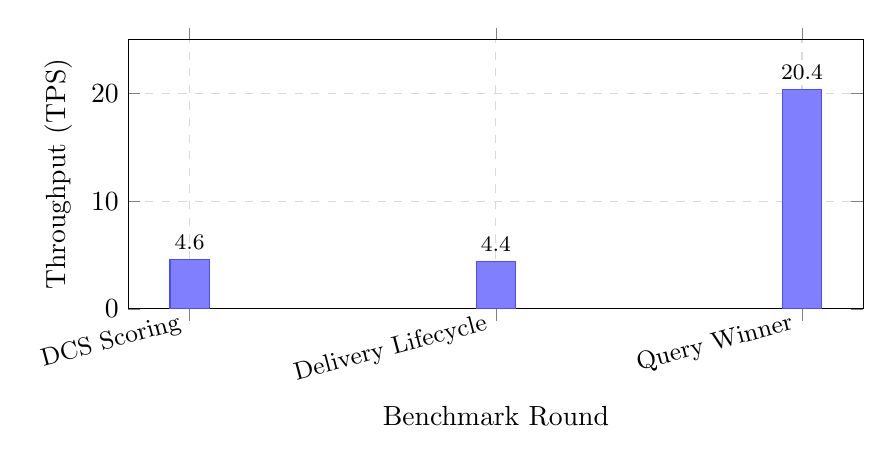
\begin{tikzpicture}
    \begin{axis}[
      ybar,
      width=0.9\columnwidth,
      height=5cm,
      bar width=0.5cm,
      xlabel={Benchmark Round},
      ylabel={Throughput (TPS)},
      symbolic x coords={DCS Scoring, Delivery Lifecycle, Query Winner},
      xtick=data,
      x tick label style={font=\small, rotate=15, anchor=east},
      ymin=0, ymax=25,
      nodes near coords,
      nodes near coords align={vertical},
      every node near coord/.append style={font=\footnotesize},
      grid=major,
      grid style={dashed,gray!30},
    ]
    \addplot[fill=blue!50, draw=blue!70] coordinates {
      (DCS Scoring, 4.6)
      (Delivery Lifecycle, 4.4)
      (Query Winner, 20.4)
    };
    \end{axis}
  \end{tikzpicture}
  \caption{Hyperledger Caliper throughput across three UOC benchmark
    rounds. All 244 transactions completed with zero failures.}
  \label{fig:caliper}
\end{figure}

\subsection{DCS Scalability Benchmark}

Figure~\ref{fig:dcs} shows DCS selection time as a function of fleet
size, measured using a multi-threaded Python simulation representing
concurrent UAV score computation.

\begin{figure}[h]
  \centering
  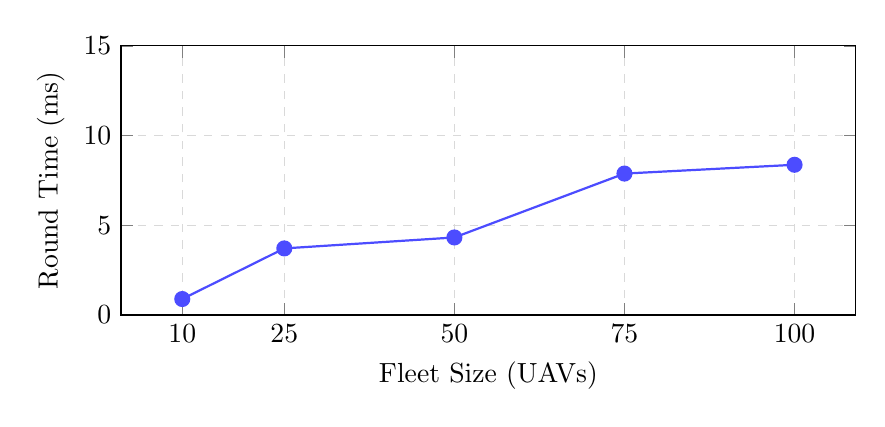
\begin{tikzpicture}
    \begin{axis}[
      xlabel={Fleet Size (UAVs)},
      ylabel={Round Time (ms)},
      width=0.9\columnwidth,
      height=5cm,
      xtick={10,25,50,75,100},
      ymin=0, ymax=15,
      mark size=2.5pt,
      grid=major,
      grid style={dashed,gray!30},
    ]
    \addplot[color=blue!70, mark=*, thick] coordinates {
      (10,  0.89)
      (25,  3.71)
      (50,  4.32)
      (75,  7.88)
      (100, 8.37)
    };
    \addplot[color=red!60, dashed, thick, domain=10:100] {140};
    \node[anchor=west, font=\small, color=red!60] at (axis cs:60,142)
      {140~ms target};
    \end{axis}
  \end{tikzpicture}
  \caption{DCS round time vs.\ fleet size. All measurements are
    94\% below the 140~ms target (red dashed line). Winner selection
    for 100~UAVs completes in 8.37~ms.}
  \label{fig:dcs}
\end{figure}

All five fleet sizes complete well below the 140~ms target, with the
100-UAV case achieving 8.37~ms --- a 16.7$\times$ margin.
Table~\ref{tab:dcs} provides the raw measurements.

\begin{table}[h]
\centering
\caption{DCS Scalability Measurements}
\label{tab:dcs}
\begin{tabular}{@{}rrc@{}}
\toprule
\textbf{Fleet Size} & \textbf{Round Time (ms)} & \textbf{$\leq$ 140~ms?} \\
\midrule
 10 &  0.89 & \checkmark \\
 25 &  3.71 & \checkmark \\
 50 &  4.32 & \checkmark \\
 75 &  7.88 & \checkmark \\
100 &  8.37 & \checkmark \\
\bottomrule
\end{tabular}
\end{table}

%% ===================================================================
\section{Conclusion and Future Work}
\label{sec:conclusion}

This paper presented DCBA, a dual-chain blockchain architecture that
simultaneously addresses pharmaceutical supply chain integrity, patient
data sovereignty, and priority-aware UAV delivery logistics. By
separating concerns across purpose-specific chains (PDC on Ethereum PoA
and UOC on Hyperledger Fabric), connected by a replay-safe cross-chain
oracle bridge, DCBA resolves the fundamental tension between patient
privacy and IoT operational throughput that prevents existing
single-chain systems from serving both domains adequately.

The implementation demonstrates that the six contributions are not
only theoretically sound but practically achievable: 86~automated
tests pass with zero failures, the DCS algorithm selects the optimal
UAV from 100 candidates in 8.37~ms (a 16.7$\times$ margin over the
140~ms target), the oracle bridge relays prescription verification in
16~ms, and all 10 adversarial test cases are blocked without false
negatives.

\textbf{Future Work.} The following extensions are identified for
subsequent research. First, decentralisation of the SC-7 oracle layer
using threshold signature aggregation (e.g., Chainlink DECO) would
eliminate the single-relay point of failure in the current testnet
implementation. Second, integration with physical UAV hardware (e.g.,
Raspberry Pi-based autopilot with hardware MAC attestation) would
validate the hardware-bound identity scheme in a real deployment
context. Third, a national-scale simulation modelling the DGDA
regulatory compliance requirements of Bangladesh would assess DCBA's
readiness for production deployment. Fourth, formal verification of
the SC-7 state machine and SC-2 consent model using tools such as
Certora Prover or Echidna would provide machine-checked security
guarantees beyond the empirical test suite. Fifth, extension of the
PARS system with a machine learning component for PARS inflation
detection would reduce dependence on manual Regulatory Auditor
monitoring.

%% ===================================================================
\begin{acks}
The authors thank the Department of Computer Science and Engineering
at Bangladesh University of Engineering and Technology (BUET) for
supporting this research. This work was conducted as part of the M.Sc.
programme at BUET, 2025--2026.
\end{acks}

%% ===================================================================
\bibliographystyle{ACM-Reference-Format}
\bibliography{references}

\end{document}
